\documentclass[fullscreen=true, bookmarks=true, hyperref={pdfencoding=unicode}]{beamer}
\usepackage[utf8]{inputenc}                                % Кодировка
\usepackage[english,russian]{babel}                        % Переносы
\usepackage{xcolor}                                        % Работа с цветом
\usepackage{amsmath,amssymb,amsfonts}                      % Символы АМО
\usepackage{graphicx}                                      % Графика
\usepackage[labelsep=period]{caption}                      % Разделитель в подписях к рисункам и таблицам
\usepackage{hhline}                                        % Для верстки линий в таблицах
\usepackage{tikz}                                          % Для простых рисунков в документе
\usepackage{fancybox}                                      % Пакет для отрисовки рамок
\usepackage{verbatim}                                      % Для вставки кода в презентацию
\usepackage{animate}                                       % Для вставки видео в презентацию
\usepackage{xmpmulti}                                      % Для вставки gif в презентацию
\usepackage{multirow}
\usepackage{mathrsfs}

\usetikzlibrary{arrows, snakes, backgrounds}                 % Для отрисовки стрелок
\usetikzlibrary{positioning, fit, arrows.meta, shapes, calc}
% used to avoid putting the same thing several times...
% Command \empt{var1}{var2}
\newcommand{\empt}[2]{$#1^{\langle #2 \rangle}$}

\graphicspath{{images/}}                                   % Путь до рисунков
\setbeamertemplate{caption}[numbered]                      % Включение нумерации рисунков

\definecolor{links}{HTML}{2A1B81}                          % blue for url links
\hypersetup{colorlinks,linkcolor=,urlcolor=links}          % nothing for others

\usetheme{boxes}
\usecolortheme{crane}

\usepackage{pythonhighlight}

\newtheorem*{question}{Вопрос}

\title{Лекция 5. Модели внимания и трансформеры}
\author{Александр Юрьевич Авдюшенко}
\institute{МКН СПбГУ}
\date{17 марта 2022}
\titlegraphic{
\includegraphics[keepaspectratio,width=0.5\textwidth]{logo_fmkn.png}}

\begin{document}
%\unitlength=2mm

% выводим заглавие
\begin{frame}
\transdissolve[duration=0.2]
\titlepage
\end{frame}


\begin{frame}
  \frametitle{Пятиминутка}
  \begin{itemize}
    \item Опишите (или нарисуйте) общую архитектуру автокодировщика
    \item Какое основное преимущество метода self-supervised learning?
    \item Выпишите функции потерь в GAN
  \end{itemize}
\end{frame}


\begin{frame}
  \frametitle{Простейшая рекуррентная нейронная сеть (vanilla RNN)}
  \framesubtitle{напоминание}

  Оставляем один скрытый вектор $h$:

  $$ h_t = f_W(h_{t-1}, x_t)$$

  В качестве функции $f_W$ задаём линейное преобразование с нелинейной <<сигмоидой>> по компонентам:

  \begin{align*}
       h_t &= \tanh ({\color{red}W_{hh}} h_{t-1} + {\color{red}W_{xh}} x_t) \\
       y_t &= {\color{red}W_{hy}} h_t
  \end{align*}

  Недостатки
  \begin{enumerate}
    \item длины входного и выходного сигнала должны совпадать
    \item «читаем» вход только слева-направо, не смотрим вперёд
    \item как следствие, не подходит для задач machine translation, question answering и т.п.
  \end{enumerate}

\end{frame}


\begin{frame}
  \frametitle{RNN для синтеза последовательностей (seq2seq)}

  $X = (x_1, \dots, x_n)$ — входная последовательность

  $Y = (y_1, \dots, y_m)$ — выходная последовательность

  ${\color{red}c \equiv h_n}$ кодирует всю информацию про $X$ для синтеза $Y$

  \begin{center}
    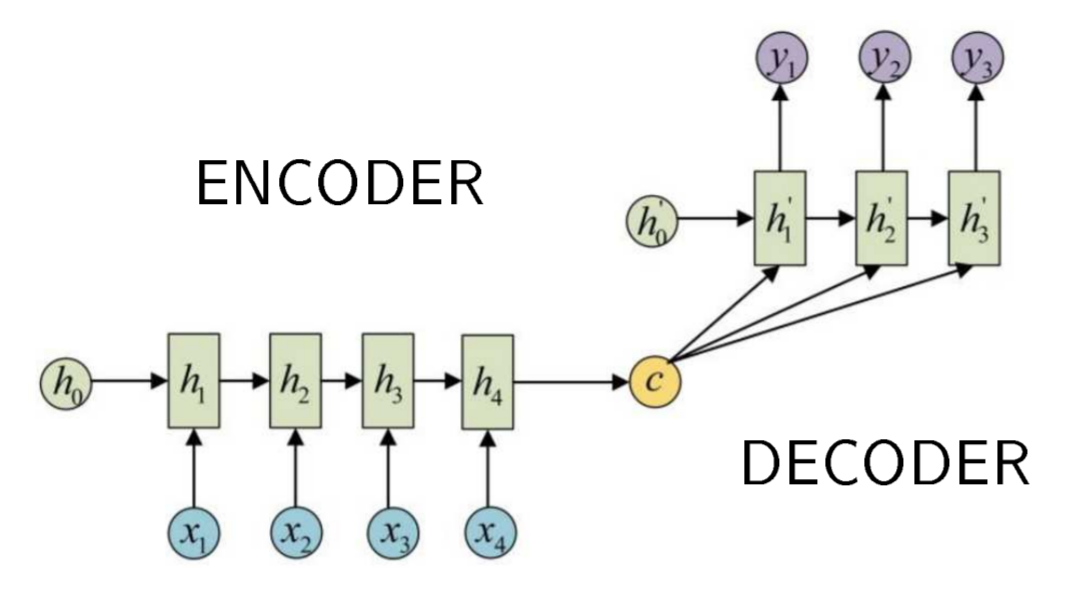
\includegraphics[keepaspectratio,
                   width=.7\paperwidth]{seq2seq.png}
  \end{center}
\end{frame}


\begin{frame}
  \begin{center}
    \begin{align*}
      h_i &= f_{in}(x_i, h_{i-1}) \\
      {\color{red}h_t^\prime} &{\color{red}= f_{out}(h_{t-1}^\prime,y_{t-1},c)} \\
      y_t &= f_{y}(h_t^\prime, y_{t-1})
    \end{align*}
  \end{center}

  \begin{itemize}
    \item $h_n$ лучше помнит конец последовательности, чем начало
    \item чем больше $n$, тем труднее упаковать всю информацию в $c$
    \item придётся контролировать затухание и взрывы градиента
    \item RNN трудно распараллеливается
  \end{itemize}
  \pause
  \begin{question}
    Как можно исправить часть перечисленных проблем?
  \end{question}
  \pause
  \begin{exampleblock}{Подсказка}
    Как люди воспринимают информацию?
  \end{exampleblock}
\end{frame}


\begin{frame}
  \frametitle{Посчитаем количество пасов}

  \href{https://www.youtube.com/watch?v=tkvtGusJt6E}{Баскетбол!}

\end{frame}


\begin{frame}
  \frametitle{RNN с вниманием (attention mechanism)}

  $a(h, h^\prime)$ — функция сходства состояний входа $h$ и выхода $h^\prime$
  (например, скалярное произведение или $\exp(h^T h^\prime)$ и другие)

  \vspace{0.5cm}
  $\alpha_{ti}$ — важность входа $i$ для выхода $t$ (attention score), $\sum_i \alpha_{ti} = 1$

  $c_t$ — вектор входного контекста для выхода $t$ (context vector)

  \begin{center}
    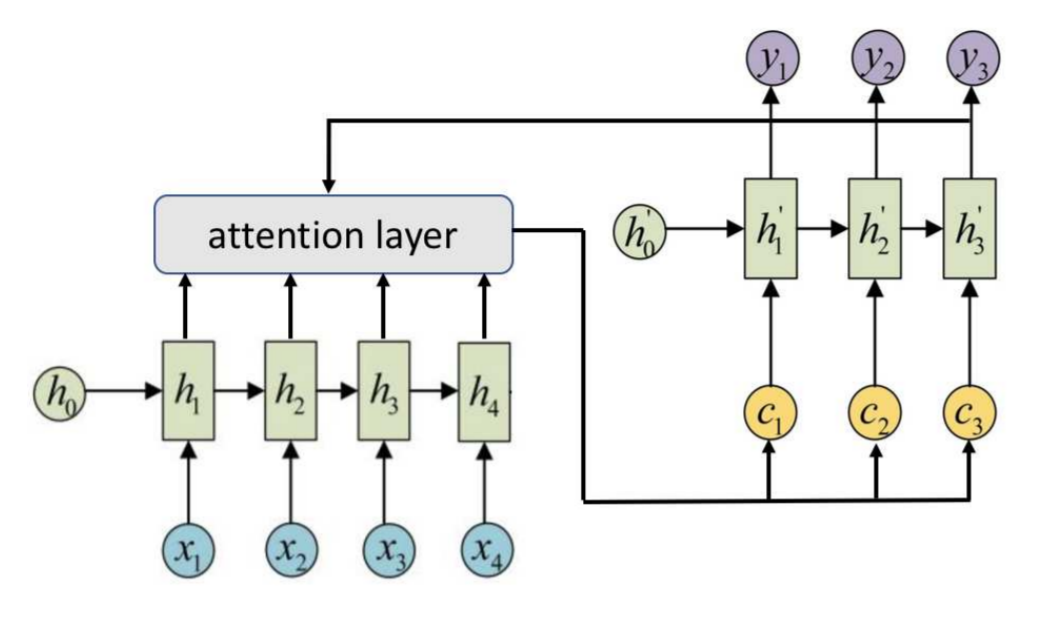
\includegraphics[keepaspectratio,
                   width=.6\paperwidth]{seq2seq_attention.png}
  \end{center}

\end{frame}


\begin{frame}

  \begin{align*}
    h_i &= f_{in}(x_i, h_{i-1}) \\
    {\color{red}\alpha_{ti}} &= \text{norm}_i a(h_i, h^\prime_{t-1}),\text{ norm}_i(p) = \frac{p_i}{\sum_j p_j} \\
    {\color{red}c_t} &= \sum_i \alpha_{ti} h_i
  \end{align*}

  \begin{align*}
   h_t^\prime &= f_{out} (h^\prime_{t-1}, y_{t-1}, {\color{red}c_t}) \\
   y_t &= f_{y}(h_t^\prime, y_{t-1}, {\color{red}c_t})
  \end{align*}

  \begin{itemize}
    \item можно вводить обучаемые параметры в $a$ и $c$
    \item можно отказаться от рекуррентности как по $h_i$, так и по $h_t^\prime$
  \end{itemize}

   \noindent\rule{8cm}{0.4pt}

  {\it Bahdanau et al.} Neural machine translation by jointly learning to align and translate. 2015
\end{frame}

\begin{frame}
  \frametitle{Применение моделей внимания}

  Преобразование одной последовательности в другую, seq2seq
  \begin{itemize}
    \item Машинный перевод
    \item Ответы на вопросы (question answering)
    \item Суммаризация текста (text summarization)
    \item Аннотация изображений, видео (multimedia description)
    \item Распознавание речи
    \item Синтез речи
  \end{itemize}

  \vspace{1cm}
  Обработка последовательности
  \begin{itemize}
    \item Классификация текстовых документов
    \item Анализ тональности документа
  \end{itemize}
 \end{frame}


\begin{frame}
  \frametitle{Внимание в машинном переводе}

  \begin{center}
    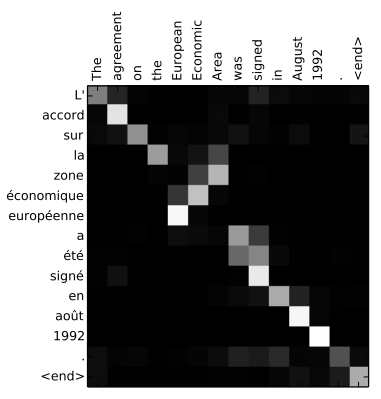
\includegraphics[keepaspectratio,
                   width=.5\paperwidth]{eng_to_french.png}

  {\small Интерпретируемость модели внимания: визуализация матрицы} $\alpha_{ti}$
  \end{center}
\end{frame}

\begin{frame}
  \frametitle{Внимание для аннотирования изображений}

  \begin{center}
    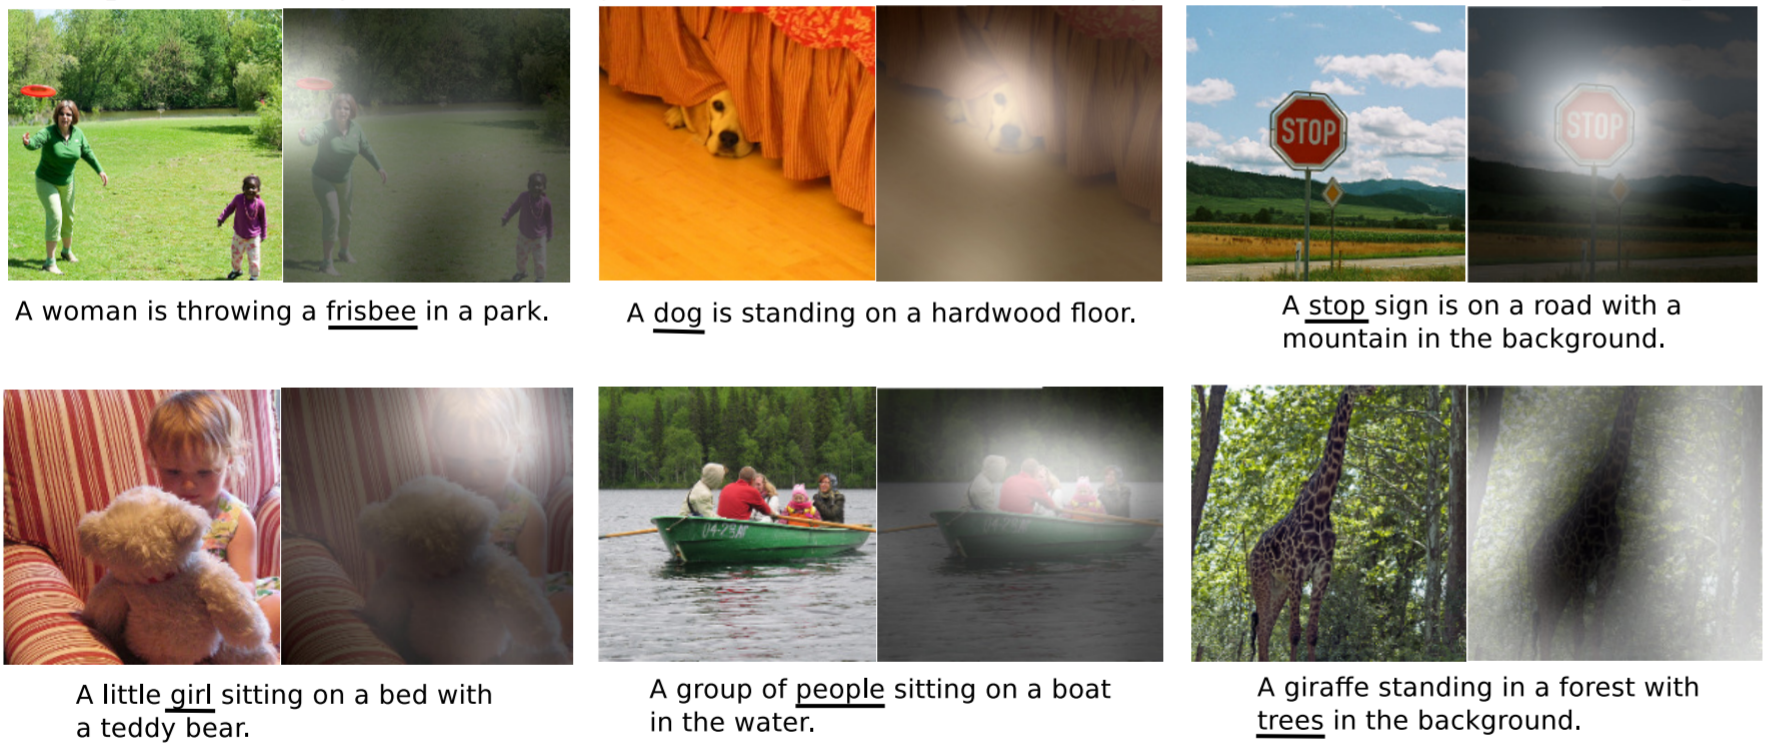
\includegraphics[keepaspectratio,
                   width=.8\paperwidth]{image_attention.png}
  \end{center}

  При генерации слова в описании изображения визуализация показывает, на какие области изображения модель обращает внимание.

  \noindent\rule{8cm}{0.4pt}

  {\small
  {\it Kelvin Xu et al.} Show, attend and tell: neural image caption generation with visual
  attention. 2016}
\end{frame}


\begin{frame}
  \frametitle{Функции сходства векторов}

        $a(h, h^\prime) = h^T h^\prime$ — скалярное произведение

        $a(h, h^\prime) = exp(h^T h^\prime)$ — norm превращается в SoftMax

        $a(h, h^\prime) = h^T {\color{red}W} h^\prime$ — с матрицей обучаемых параметров $\color{red}{W}$

        $a(h, h^\prime) = {\color{red}w^T} \tanh ({\color{red}U}h + {\color{red}V} h^\prime)$ — аддитивное внимание с ${\color{red}w, U, V}$

        \vspace{0.5cm}
        {\bf Линейные преобразования векторов} query, key, value:

    \begin{columns}
      \begin{column}{.6\paperwidth}
        $a(h_i, h^\prime_{t-1}) = ({\color{red}W_k}h_i)^T ({\color{red}W_q}h^\prime_{t-1}) / \sqrt{d}$

        $\alpha_{ti} = \text{SoftMax}_i a(h_i, h^\prime_{t-1})$

        $c_t = \sum\limits_i \alpha_{ti} {\color{red}W_v} h_i $

        ${\color{red}W_q}_{d \times dim(h^\prime)}, {\color{red}W_k}_{d \times dim(h)}, {\color{red}W_v}_{d \times dim(h)}$ — матрицы весов линейных нейронов

        Возможно упрощение ${\color{red}W_k} \equiv {\color{red}W_v}$
        {\footnotesize
        \noindent\rule{8cm}{0.4pt}

        {\it Dichao Hu.} An introductory survey on attention mechanisms in NLP problems. 2018}
      \end{column}
      \begin{column}{.18\paperwidth}
        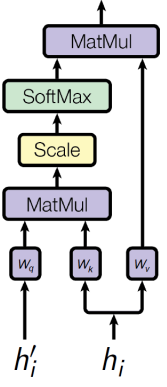
\includegraphics[keepaspectratio,
                       width=.15\paperwidth]{general_attention.png}
      \end{column}
  \end{columns}

\end{frame}


\begin{frame}
  \frametitle{Формула внимания}

  $q$ — вектор-запрос, для которого хотим вычислить контекст

  $K = (k_1, \dots, k_n)$ — векторы-ключи, сравниваемые с запросом

  $V = (v_i, \dots, v_n)$ — векторы-значения, образующие контекст

  $a(k_i, q)$ — оценка релевантности (сходства) ключа $k_i$ запросу $q$

  $c$ — искомый вектор контекста, релевантный запросу

  {\small
  \begin{block}{Модель внимания}
   Это 3х-слойная сеть, вычисляющая выпуклую комбинацию значений $v_i$, релевантных запросу $q$:

   $$ c = Attn(q,K,V) = \sum\limits_i v_i \text{SoftMax}_i a(k_i, q) $$
 \end{block}
 }

  $c_t = Attn({\color{red}W_q} h^\prime_{t-1}, {\color{red}W_k} H, {\color{red}W_v} H)$ — пример с предыдущего слайда, где $H = (h_1, \dots, h_n)$ — входные векторы, $h^\prime_{t-1}$ — выходной


  Внутреннее внимание или «самовнимание» (self-attention):

  $c_i = Attn({\color{red}W_q} h_{i}, {\color{red}W_k} H, {\color{red}W_v} H)$ — частный случай, когда $h^\prime \in H$
\end{frame}


\begin{frame}
  \frametitle{Многомерное внимание (multi-head attention)}

  {\bf Идея}: $J$ разных моделей внимания совместно обучаются выделять различные аспекты входной информации (например, части речи, синтаксис, фразеологизмы):

  $ c^j = \text{Attn}({\color{red}W^j_q} q, {\color{red}W^j_k} H, {\color{red}W^j_v} H), j = 1, \dots, J$

  {\bf Варианты} агрегирования выходного вектора:

  $ c = \frac{1}{J} \sum\limits_{j=1}^J c^j$ — усреднение

  $ c = [c^1 \dots c^J]$ — конкатенация

  $ c = [c^1 \dots c^J] {\color{red}W}$ — чтобы вернуться к нужной размерности

  {\bf Регуляризация}: чтобы аспекты внимания были максимально различны, строки $J \times n$ матриц $A, \alpha_{ji} = \text{SoftMax}_i a({\color{red}W_k^j}h_i, {\color{red}W_q^j}q)$, декоррелируются $(\alpha_{s}^T\alpha_{j} \to 0)$ и разреживаются $(\alpha_{j}^T\alpha_{j} \to 1)$:

  $$\|AA^T - I \|^2 \to \min\limits_{\{{\color{red}W_k^j}, {\color{red}W_q^j}\}} $$

  \noindent\rule{8cm}{0.4pt}

  {\small
  {\it Zhouhan Lin, Y.Bengio et al}. A structured self-attentive sentence embedding. 2017}
\end{frame}


\begin{frame}
  \frametitle{Не рассматриваем подробно в этой лекции}

  \begin{itemize}
    \item иерархическое внимание (например, для классификации документов):  слова  $\in$ предложения $\in$ документы
    \item Graph Attention Network (GAT): многоклассовая multi-label классификация вершин графа
  \end{itemize}
  \vspace{2cm}

  \noindent\rule{8cm}{0.4pt}

  {\small
  {\it Z.Yang, A.Smola et al.} Hierarchical attention networks for document classification. 2016

  {\it Petar Velickovic et al.} Graph Attention Networks. ICLR-2018}
\end{frame}


{ % all template changes are local to this group.
    \setbeamertemplate{navigation symbols}{}
    \begin{frame}<article:0>[plain]
        \begin{tikzpicture}[remember picture,overlay]
            \node[at=(current page.center)] {
                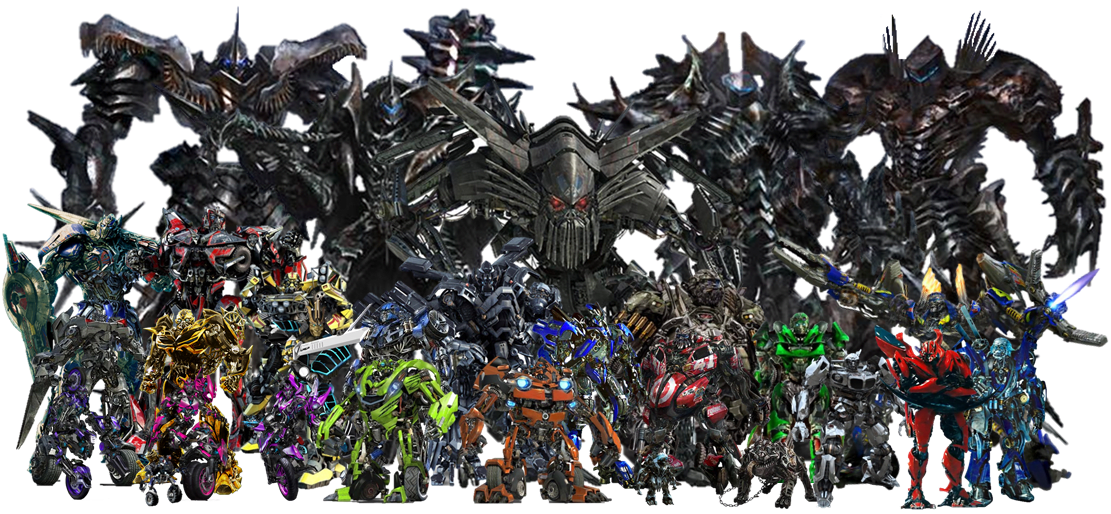
\includegraphics[keepaspectratio,
                                 width=\paperwidth,
                                 height=\paperheight]{many_transformers.png}
            };
        \end{tikzpicture}
     \end{frame}
}


\begin{frame}
  \frametitle{Трансформер для машинного перевода}

  Трансформер (transformer) — это нейросетевая архитектура на основе моделей внимания и полносвязных слоёв, без RNN

  Схема преобразований данных в машинном переводе:

  \begin{itemize}
    \item $S = (w_1, \dots, w_n)$ — слова предложения на входном языке

          $\downarrow$ обучаемая или пред-обученная векторизация слов $\downarrow$
    \item $X = (x_1, \dots, x_n)$ — эмбединги слов входного предложения

          $\downarrow$ трансформер-кодировщик $\downarrow$
    \item $Z = (z_1, \dots, z_n)$ — контекстные эмбединги

          $\downarrow$ трансформер-декодировщик $\downarrow$
    \item $Y = (y_1, \dots, y_m)$ — эмбединги слов выходного предложения

          $\downarrow$ генерация слов из построенной языковой модели $\downarrow$
    \item $\tilde S = (\tilde w_1, \dots, \tilde w_m)$ — слова предложения на выходном языке
  \end{itemize}

  \noindent\rule{8cm}{0.4pt}

  {\small
  {\it Vaswani et al.} (Google) Attention is all you need. 2017}
\end{frame}


{ % all template changes are local to this group.
    \setbeamertemplate{navigation symbols}{}
    \begin{frame}<article:0>[plain]
        \begin{tikzpicture}[remember picture,overlay]
            \node[at=(current page.center)] {
                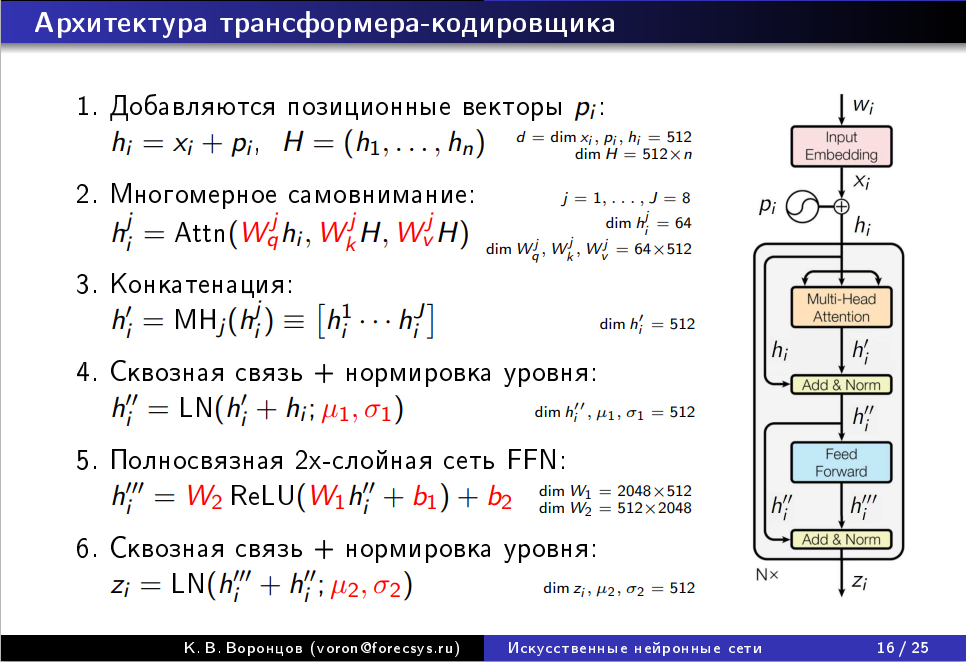
\includegraphics[keepaspectratio,
                                 width=\paperwidth,
                                 height=\paperheight]{transformer_scheme.png}
            };
        \end{tikzpicture}
     \end{frame}
}


\begin{frame}
  \frametitle{Дополнения и замечания}

   \begin{itemize}
     \item ещё таких блоков $N=6, h_i \to \square \to z_i$ соединены последовательно
     \item вычисления легко распараллеливаются по $x_i$
     \item возможно использование пред-обученных эмбедингов $x_i$
     \item возможно обучение эмбедингов $x_i$ слов $w_i \in V$
     \item слой нормировки уровня (Layer Normalization, LN), $x, {\color{red}\mu}, {\color{red}\sigma} \in \mathbb{R}^d$
   \end{itemize}

   \begin{align*}
     LN_s(x; {\color{red}\mu}, {\color{red}\sigma}) = {\color{red}\sigma_s} \frac{x_s - \overline{x}}{\sigma_x} + {\color{red}\mu_s} \\
     \overline{x} = \frac{1}{d} \sum\limits_{s=1}^d x_s, \sigma_x^2 = \frac{1}{d} \sum\limits_{s=1}^d (x_s - \overline{x})
   \end{align*}
 \end{frame}


\begin{frame}
  \frametitle{Позиционное кодирование (positional encoding)}

  Позиции слов $i$ кодируются векторами $p_i$ так, что
  \begin{itemize}
    \item чем больше $|i-j|$, тем больше $\|p_i-p_j\|$
    \item число позиций не ограничено
  \end{itemize}

  Например,

  $ c_j = \text{Attn}(q_j, K, V) = \sum_i (v_i + {\color{red}w^v_{i\boxminus j}}) \text{SoftMax}_i a(k_i + {\color{red} w^k_{i\boxminus j}}, q_j), $

  где $i\boxminus j = \max(\min(i-j, \delta), -\delta)$ — усеченная разность, $\delta = 5..16$

  \vspace{1cm}
  \noindent\rule{8cm}{0.4pt}

  {\small
  {\it Shaw, Uszkoreit, Vaswani.} Self-attention with relative position representations. 2018}
\end{frame}


{ % all template changes are local to this group.
    \setbeamertemplate{navigation symbols}{}
    \begin{frame}<article:0>[plain]
        \begin{tikzpicture}[remember picture,overlay]
            \node[at=(current page.center)] {
                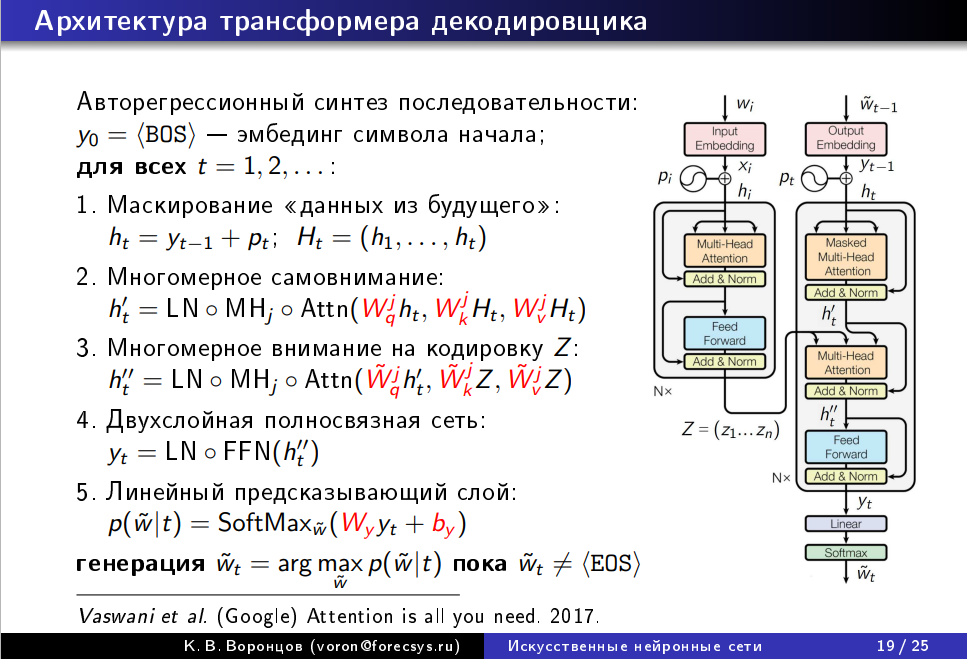
\includegraphics[keepaspectratio,
                                 width=\paperwidth,
                                 height=\paperheight]{transformer_scheme_2.png}
            };
        \end{tikzpicture}
     \end{frame}
}


\begin{frame}
  \frametitle{Критерии обучения и валидации для машинного перевода}

  {\bf Критерий для обучения} параметров нейронной сети $\color{red}{W}$ по обучающей выборке предложений $S$ c переводом $\tilde S$:

  $$ \sum\limits_{(S, \tilde S)} \sum\limits_{\tilde w_t \in \tilde S} \ln p(\tilde w_t|t, S, {\color{red}W}) \to \max\limits_W $$

  {\bf Критерий оценивания моделей} (недифференцируемый) по выборке пар предложений «перевод $S$, эталон $S_0$»:

  BiLingual Evaluation Understudy:

  \begin{align*}
    \text{BLEU} &= \min \left(1, \frac{\sum \text{len}(S)}{\sum \text{len}(S_0)} \right) \times \\
    \underset{(S_0, S)}{\text{mean}}&\left(\prod\limits_{n=1}^4 \frac{\#n\text{-грамм из } S, \text{входящих в } S_0}{\#n\text{-грамм в } S} \right)^{\frac14}
  \end{align*}
\end{frame}


{ % all template changes are local to this group.
    \setbeamertemplate{navigation symbols}{}
    \begin{frame}<article:0>[plain]
        \begin{tikzpicture}[remember picture,overlay]
            \node[at=(current page.center)] {
                
\includegraphics[keepaspectratio,
                                 width=\paperwidth,
                                 height=\paperheight]{BERT_real.png}
            };
        \end{tikzpicture}
     \end{frame}
}


\begin{frame}
  \frametitle{BERT — Bidirectional Encoder Representations from Transformers}

  Трансформер BERT — это кодировщик без декодировщика, предобучаемый для решения широкого класса задач NLP

  Схема преобразований данных в задачах NLP:

  \begin{itemize}
    \item $S = (w_1, \dots, w_n)$ — слова предложения на входном языке

          $\downarrow$ обучение эмбедингов вместе с трансформером $\downarrow$
    \item $X = (x_1, \dots, x_n)$ — эмбединги слов входного предложения

          $\downarrow$ трансформер-кодировщик $\downarrow$
    \item $Z = (z_1, \dots, z_n)$ — контекстные эмбединги

          $\downarrow$ дообучение на конкретную задачу $\downarrow$
    \item $Y$ — выходной текст / разметка / классификация и т.п.
  \end{itemize}

  \noindent\rule{8cm}{0.4pt}

  {\small
  {\it Jacob Devlin, Ming-Wei Chang, Kenton Lee, Kristina Toutanova} (Google AI Language)
  BERT: pre-training of deep bidirectional transformers for language understanding. 2019.}
\end{frame}


\begin{frame}
  \frametitle{Критерий MLM (masked language modeling) для обучения BERT}

  Критерий маскированного языкового моделирования MLM строится автоматически по текстам (self-supervised learning):

  $$ \sum\limits_{S} \sum\limits_{ i \in M(S)} \ln p(w_i|i, S, {\color{red}W}) \to \max\limits_W, $$

  где $M(S)$ — подмножество маскированных токенов из $S$,

  $$ p(w|i, S, {\color{red}W}) = \underset{w \in V}{\text{SoftMax}}({\color{red}W_z}z_i(S, {\color{red}W_T}) + {\color{red}b_z})$$

  — языковая модель, предсказывающая $i$-й токен предложения $S$, $z_i(S, {\color{red}W_T})$ — контекстный эмбединг $i$-го токена предложения $S$ на выходе трансформера с параметрами ${\color{red}W_T}$,

  ${\color{red}W}$ — все параметры трансформера и языковой модели
\end{frame}


\begin{frame}
  \frametitle{Критерий NSP (next sentence prediction) для обучения BERT}

  Критерий предсказания связи между предложениями NSP строится автоматически по текстам (self-supervised learning):

  $$ \sum\limits_{(S, S^\prime)} \ln p\left(y_{SS^\prime}|S, S^\prime, {\color{red}W}\right) \to \max\limits_W, $$

  где $y_{SS^\prime} = $ [за $S$ следует $S^\prime$] — бинарная классификация пары предложений,

  $$ p(y|S, S^\prime, {\color{red}W}) = \underset{y \in \{0,1\}}{\text{SoftMax}}\left({\color{red}W_y} \tanh({\color{red}W_s}z_0(S, S^\prime, {\color{red}W_T}) + {\color{red}b_s}) + {\color{red}b_y}\right)$$

  — вероятностная модель классификации пар $(S, S^\prime)$, $z_0(S, S^\prime, {\color{red}W_T})$ — контекстный эмбединг токена  $\left<\text{CLS}\right>$ для пары предложений, записанной в виде $\left<\text{CLS}\right> S \left<\text{SEP}\right> S^\prime \left<\text{SEP}\right>$
\end{frame}


\begin{frame}
  \frametitle{Ещё несколько замечаний про трансформеры}

  \begin{itemize}
    \item Fine-tuning: для дообучения на задаче задаётся модель $f(Z(S, {\color{red}W_T}), {\color{red}W_f})$, выборка $\{S\}$ и критерий $\mathcal{L}(S, f) \to \max$
    \item Multi-task learning: для дообучения на наборе задач $\{t\}$ задаются модели $f_t(Z(S, {\color{red}W_T}), {\color{red}W_f})$, выборки $\{S\}_t$ и сумма критериев $ \sum_t \lambda_t \sum_S \mathcal{L}_t(S, f_t) \to \max $
    \item GLUE, SuperGLUE, Russian SuperGLUE — наборы тестовых задач на понимание естественного языка
    \item Трансформеры обычно строятся не на словах, а на токенах, получаемых BPE (Byte-Pair Encoding) или WordPiece
    \pause
    \item Первый трансформер: $N = 6, d = 512, J = 8$, весов 65M
    \item $\text{BERT}_{\text{BASE}}$, GPT-1: $N = 12, d = 768, J = 12$, весов 110M
    \item $\text{BERT}_{\text{LARGE}}$, GPT-2: $N = 24, d = 1024, J = 16$, весов 340M-1000M
    \pause
    \item GPT-3: весов 175 млрд
    \item Gopher (DeepMind): 280 млрд
    \item Turing-Megatron (Microsoft + Nvidia): 530 млрд
  \end{itemize}
\end{frame}


\begin{frame}
  \frametitle{Резюме}
  \begin{itemize}
    \item Модели внимания сначала встраивались в RNN или CNN, но оказалось, что они самодостаточны
    \item На их основе разработана архитектура Трансформера, различные варианты которого (BERT, GPT-3, XLNet, ELECTRA и др.) на данный момент являются SotA в задачах обработки естественного языка, и не только его
    \item Доказано, что модель внимания multi-head self-attention (MHSA) эквивалентна свёрточной сети [Cordonnier, 2020]
  \end{itemize}

  \noindent\rule{8cm}{0.4pt}

  {\small
  {\it Vaswani et al.} Attention is all you need. 2017.

  {\it Dichao Hu.} An Introductory Survey on Attention Mechanisms in NLP Problems. 2018.

  {\it Xipeng Qiu et al.} Pre-trained models for natural language processing: A survey. 2020.

  {\it Cordonnier et al.} On the relationship between self-attention and convolutional layers. 2020}
\end{frame}


\begin{frame}
  Что ещё можно посмотреть?
  \begin{itemize}
    \item Лекция К.В. Воронцова \href{https://www.youtube.com/watch?v=KhMweP00S44}{«Модели внимания и трансформеры»}
    \item GPT-3 на википедии: \href{https://en.wikipedia.org/wiki/GPT-3}{https://en.wikipedia.org/wiki/GPT-3}
    \item Григорий Сапунов \href{https://www.youtube.com/watch?v=8dN6ZVnDArk&t}{о трансформерах в 2021}
    \item Николай Григорьев (SE @ Deepmind) \href{https://www.youtube.com/watch?v=8Q-a6-P6Eyo}{об истории и современных языковых моделях}, 14 февраля 2022
    \item \href{https://disk.yandex.ru/d/knoQ44wLmGDwwQ}{Семинар ММЦ Эйлера и МКН о формализации математических доказательств в Lean и глубоком обучении}
  \end{itemize}
\end{frame}

\end{document}
